%-----------------------------------------------------------
Moja práca na hardvérovej časti tímového projektu -- návrh
\textit{mechanickej konštrukcie} a \textit{geometrický vzťah medzi
referenčnými rámcami senzorov}

%-----------------------------------------------------------
\section{Hardvérové komponenty a ich úloha}
Platforma integruje tri senzorické zariadenia, výpočtovú jednotku, a~mikroelektroniku
zabezpečujúcu komunikáciu, mechanicky zviazané do
jedného tuhého celku pomocou hliníkového profilu a~3D-tlačených konštrukčných dielov:

\begin{itemize}
  \item \textbf{LiDAR Hesai XT16} -- primárny zdroj 3D geometrie scény (16~kanálov,
        rotujúci skener). Definuje hlavný (referenčný) súradnicový systém modulu, do
        ktorého sú ostatné senzory kalibrované.
  \item \textbf{IMU ICM-40609-D} -- 6-DoF inerciálna jednotka so známym počiatkom súradnicovej sústavy
        (akcelerometrický origin). Slúži na určenie orientácie a~pomáha pri
        synchronizácii LiDAR-ových mračien bodov.
  \item \textbf{Kamera Basler a2A 1920 - 160uc PRO} so~6\,mm C-mount objektívom -- vizuálny kanál
        pre fúziu s~LiDAR-om (textúra a ofarbenie mračna bodov).
  \item \textbf{Jetson AGX Orin 64GB} -- výpočtová jednotka, mechanicky odsadená od
        senzorického modulu (vlastný 3D-tlačený box).
  \item \textbf{Akumulátor Amewi Li-Pol 5500mAh/14,8V} -- umiestnená v boxe s~GPU, napája GPU a LiDAR.
  \item \textbf{STM32 F103 Bluepill} -- mikrokontrolér pre synchronizáciu a komunikáciu senzorov
  \item \textbf{TTL/RS232 prevodník} -- zabezpečuje komunikáciu mikrokontroléra s LiDARom

\end{itemize}

Nosnou kostrou je hliníkový profil spájaný drážkovými T-maticami a~zápustnými skrutkami M5.

%-----------------------------------------------------------
\section{3D modely a~mechanická koncepcia}
Konštrukcia bola navrhnutá tak, aby minimalizovala neurčitosti v~polohách senzorov
a~ostala vyrobiteľná na bežnej FDM tlačiarni. Senzorický modul je tvorený dvoma hlavnými dielmi:
spodná konzola s~kamerou a kotvením na profil a~vrchná časť s~otvormi pre LiDAR a jeho komunikačný box.
Bočnice (steny) uzatvárajú modul. GPU spolu s baterkou sú umiestnené v~oddelenom
boxe, ktorý je uchytený L konzolami k hliníkovému profilu, čo umožňuje
servis bez rozoberania senzorickej hlavy. \textbf{Všetky tlačené súčiastky sú z materiálu PLA}.

\begin{figure}[H]
  \centering
  % --- MIESTO PRE OBRÁZOK 1: finálna konštrukcia ---
  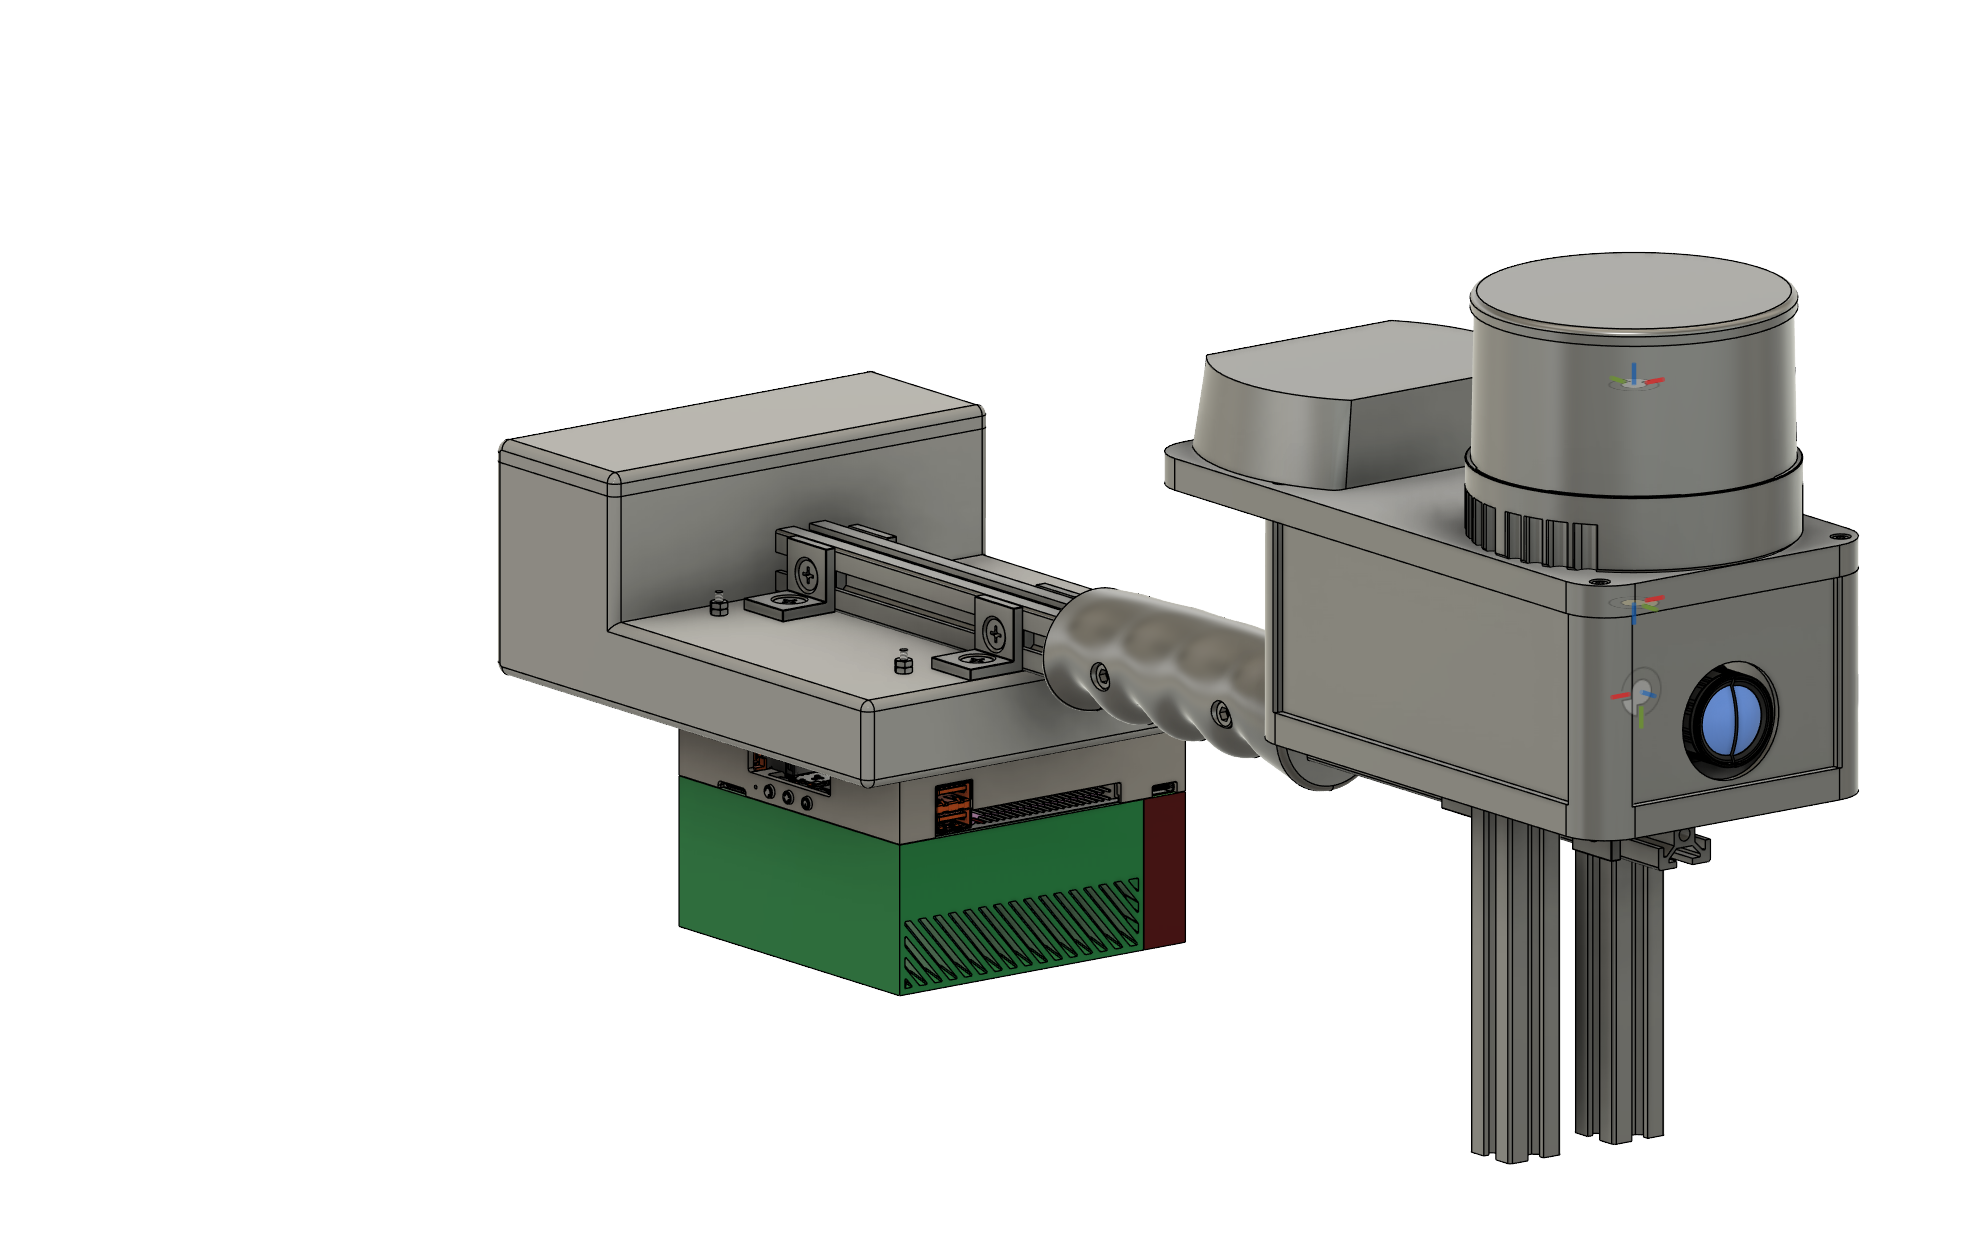
\includegraphics[width=0.62\linewidth]{../full_assembly.png}
  \caption{Finálna konštrukcia}
  \label{fig:assembly}
\end{figure}

Kľúčové dizajnové rozhodnutia: (i) LiDAR nad kamerou s~vertikálnym odsadením,
aby si zorné polia navzájom neclonili; (ii) IMU pripevnená na vrchnej časti senzorického modulu -- fixný
vzťah IMU--LiDAR bez pohyblivých spojení; (iii) Jetson v~samostatnom boxe mimo senzorickej
hlavy.

%-----------------------------------------------------------
\section{Transformácie medzi súradnicovými systémami}
Pre fúziu dát musí byť každé meranie
prevedené do jedného referenčného rámca -- zvolili sme \emph{LiDAR-rámec} $\mathcal{F}_L$.

\begin{figure}[H]
  \centering
  % --- MIESTO PRE OBRÁZOK 2: schéma transformácií medzi senzormi ---
  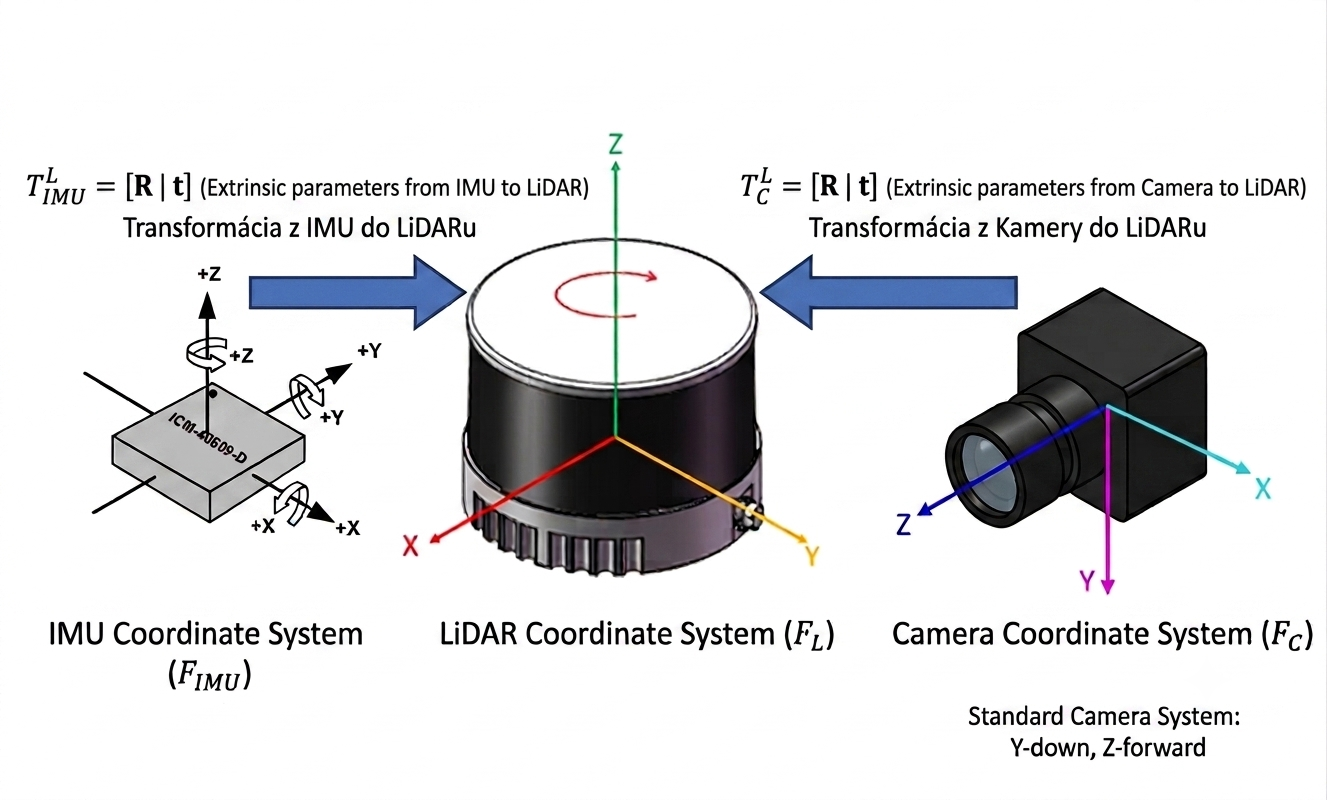
\includegraphics[width=0.8\linewidth]{../transformations.png}
  \caption{Transformácie medzi rámcami kamery~$\mathcal{F}_C$, IMU~$\mathcal{F}_I$
  a~LiDAR-u~$\mathcal{F}_L$.}
  \label{fig:transforms}
\end{figure}

\paragraph{IMU $\rightarrow$ LiDAR}
\[
\mathbf{R}_{LI}=\!\begin{bmatrix}-1 & 0 & 0\\ 0 & 1 & 0\\ 0 & 0 & -1\end{bmatrix}\!,
\qquad
\mathbf{t}_{LI}=\!\begin{bmatrix}0\\ 0\\ -0{,}06955\end{bmatrix}\!\text{m}.
\]
Rotácia zodpovedá otočeniu o~$180^\circ$ okolo osi~$y$ (IMU je voči LiDAR-u prevrátený
zhora-nadol). Posun je iba vo vertikále -- IMU sa nachádza pribl. 70\,mm pod
referenčným bodom LiDAR-u.

\paragraph{Kamera $\rightarrow$ LiDAR}
\[
\mathbf{R}_{LC}=\!\begin{bmatrix}-1 & 0 & 0\\ 0 & 0 & -1\\ 0 & -1 & 0\end{bmatrix}\!,
\qquad
\mathbf{t}_{LC}=\!\begin{bmatrix}0\\ 0{,}09590\\ -0{,}00382\end{bmatrix}\!\text{m}.
\]
$\mathbf{R}_{LC}$ rotuje rámec kamery na rámec LiDAR-u ($x_C\!\to\!-x_L$, $z_C\!\to\!-y_L$,
$y_C\!\to\!-z_L$); kamera je odsadená pribl. 96\,mm v osi y a~mierne posunutá o -3.819 mm v osi z.

%-----------------------------------------------------------
\section{Záver}
Výsledkom je tuhá modulárna konštrukcia geometricky fixujúca LiDAR, kameru a~IMU s~jasne
definovanou extrinsikou. Transformačné matice vychádzajú z~CAD geometrie a~vstupujú do senzorickej
fúzie.
